\documentclass[12pt,a4paper]{article}

% 导入必要的宏包
\usepackage[UTF8]{ctex}
\usepackage{geometry}
\usepackage{amsmath}
\usepackage{amsfonts}
\usepackage{amssymb}
\usepackage{graphicx}
\usepackage{enumitem}
\usepackage{xcolor}
\usepackage{tikz}
\usepackage{float}
\usepackage{hyperref}
\usepackage{multicol}
\usepackage{longtable}
\usepackage{array}
\usepackage{tabularx}
\usepackage{listings}

% 代码高亮设置
\lstset{
    basicstyle=\ttfamily\small,
    keywordstyle=\color{blue},
    commentstyle=\color{green!70!black},
    stringstyle=\color{red},
    breaklines=true,
    numbers=left,
    numberstyle=\tiny\color{gray},
}

% 页面设置
\geometry{left=2.5cm,right=2.5cm,top=2.5cm,bottom=2.5cm}

% 标题页设置
\title{\textbf{2017年数据结构题库} \\ \large 单项选择题与综合应用题详解}
\author{}
\date{}

% 定义题型环境
\newenvironment{choicequestion}[1][]{%
    \vspace{0.5cm}
    \noindent\textbf{[#1]}
    \vspace{0.2cm}
}{}

\newenvironment{answersection}{%
    \vspace{0.2cm}
    \noindent\textbf{[参考答案]}\\
    \vspace{0.1cm}
}{}

\newenvironment{analysissection}{%
    \vspace{0.2cm}
    \noindent\textbf{[答案解析]}\\
    \vspace{0.1cm}
}{}

% 定义题号计数器
\newcounter{questioncounter}

% 定义题号计数器
\newcounter{questioncounter}

% 问题格式化命令
\newcommand{\question}[2]{%
    \stepcounter{questioncounter}%
    \noindent\textbf{\thequestioncounter} #1%
}

% 选择题选项格式
\newcommand{\choices}[4]{%
    \begin{multicols}
    \noindent \textbf{A.} #1 \par
    \noindent \textbf{B.} #2 \par
    \noindent \textbf{C.} #3 \par
    \noindent \textbf{D.} #4 \par
    \end{multicols}%
}

% 开始文档
\begin{document}

\maketitle

\section{单项选择题}

\begin{choicequestion}[单选题]
\question{下列函数的时间复杂度是
\begin{lstlisting}[language=C]
int func(int n){
    int i = 0, sum = 0;
    while(sum < n) sum += ++i;
    return i;
}
\end{lstlisting}}{}

\choices{O(\log n)}{O(n^{1/2})}{O(n)}{O(n \log n)}

\begin{answersection}
B. O(n^{1/2})
\end{answersection}

\begin{analysissection}
循环中sum累加1+2+…+i，直到sum≥n，即i(i+1)/2≥n，解得i≈√(2n)。循环执行次数为O(√n)，即O(n^{1/2})。
\end{analysissection}
\end{choicequestion}

\begin{choicequestion}[单选题]
\question{下列关于栈的叙述中，错误的是\newline
I. 采用非递归方式重写递归程序时必须使用栈\newline
II. 函数调用时，系统要用栈保存必要的信息\newline
III. 只要确定了入栈次序，就可确定出栈次序\newline
IV. 栈是一种受限的线性表，允许在其两端进行操作}{}

\choices{仅I}{仅II、III}{仅III、IV}{仅II、III、IV}

\begin{answersection}
C. 仅III、IV
\end{answersection}

\begin{analysissection}
I正确（多数情况下需要栈保存调用信息）。  
II正确（函数调用使用栈保存返回地址和局部变量）。  
III错误（出栈次序取决于具体的入栈、出栈操作序列，而非仅入栈次序）。  
IV错误（栈只允许在一端进行操作，不是两端）。  
故错误的是III、IV。
\end{analysissection}
\end{choicequestion}

\begin{choicequestion}[单选题]
\question{适用于压缩存储稀疏矩阵的两种存储结构是}{}

\choices{三元组表和十字链表}{三元组表和邻接矩阵}{十字链表和二叉链表}{邻接矩阵和十字链表}

\begin{answersection}
A. 三元组表和十字链表
\end{answersection}

\begin{analysissection}
稀疏矩阵非零元素较少，三元组表存储非零元素的行列值和数值，十字链表是链式存储稀疏矩阵的有效结构。邻接矩阵和二叉链表不适合稀疏矩阵的压缩存储。
\end{analysissection}
\end{choicequestion}

\begin{choicequestion}[单选题]
\question{要使一棵非空二叉树的先序序列与中序序列相同，其所有非叶结点须满足的条件是}{}

\choices{只有左子树}{只有右子树}{结点的度均为1}{结点的度均为2}

\begin{answersection}
B. 只有右子树
\end{answersection}

\begin{analysissection}
先序序列为“根-左-右”，中序序列为“左-根-右”。要使二者相同，必须不存在左子树，即所有非叶结点都只有右子树。
\end{analysissection}
\end{choicequestion}

\begin{choicequestion}[单选题]
\question{已知一棵二叉树的树形如右图所示，其后序序列为e,a,c,b,d,g,f，树中与结点a同层的结点是}{}

\begin{figure}[H]
\centering
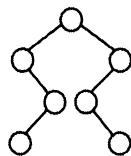
\includegraphics[width=0.3\textwidth]{images/c05cd13cde2377711d109a30d68490142d472f5cb85f10bb05acecdd18591b70.jpg}
\end{figure}

\choices{c}{d}{f}{g}

\begin{answersection}
B. d
\end{answersection}

\begin{analysissection}
后序序列e,a,c,b,d,g,f表明树结构为：a是根，e是a的左子树根，b是a的右子树根，c是b的左子树，d是b的右子树，g是d的左子树，f是d的右子树。a所在层为第1层，d与a同层（均为第2层）。
\end{analysissection}
\end{choicequestion}

\begin{choicequestion}[单选题]
\question{已知字符集 $\{a, b, c, d, e, f, g, h\}$ ，若各字符的哈夫曼编码依次是0100,10,0000,0101,001,011,11,0001，则编码序列0100011001001011110101 的译码结果是}{}

\choices{acgabfh}{adbagbb}{afbeagd}{afeefgd}

\begin{answersection}
C. afbeagd
\end{answersection}

\begin{analysissection}
按哈夫曼编码表逐段匹配：
0100 → a，011 → f，0100 → a，10 → b，001 → e，0101 → d。
译码结果为afbeagd。
\end{analysissection}
\end{choicequestion}

\begin{choicequestion}[单选题]
\question{已知无向图G含有16条边，其中度为4的顶点个数为3，度为3的顶点个数为4，其他顶点的度均小于3。图G所含的顶点个数至少是}{}

\choices{10}{11}{13}{15}

\begin{answersection}
B. 11
\end{answersection}

\begin{analysissection}
由握手定理，所有顶点度数之和为2×16=32。  
度为4的顶点贡献3×4=12，度为3的顶点贡献4×3=12，剩余度数总和为32-24=8。  
剩余顶点度数≤2，为使顶点数最少，应让剩余顶点度数尽可能大（均为2），则剩余顶点数为8/2=4。  
总顶点数至少为3+4+4=11。
\end{analysissection}
\end{choicequestion}

\begin{choicequestion}[单选题]
\question{下列二叉树中，可能成为折半查找判定树（不含外部结点）的是}{}

\begin{figure}[H]
\centering
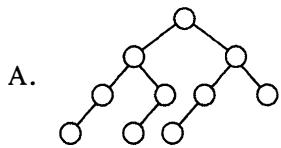
\includegraphics[width=0.3\textwidth]{images/bb494d18ea241c8803e702462b451118a8151949fb4c02c9c967d1abba026a40.jpg}
\end{figure}

\begin{figure}[H]
\centering
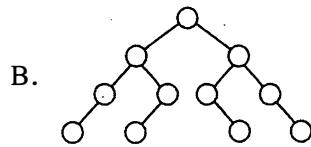
\includegraphics[width=0.3\textwidth]{images/3e503691fda84cf6b9a460cfdca33fbd99b1e080e49518f80d2e373e11841b1b.jpg}
\end{figure}

\begin{figure}[H]
\centering
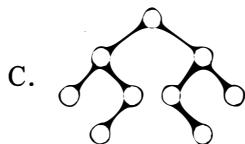
\includegraphics[width=0.3\textwidth]{images/4866ec4779e4f229f4cf4b323f630b72e2eb4b94f06427c92b129eff6c34eb1e.jpg}
\end{figure}

\begin{figure}[H]
\centering
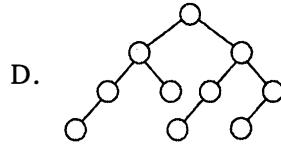
\includegraphics[width=0.3\textwidth]{images/98bc79bc9a5dc23c0681b5c568338180c8634b6a0b8849a1d54844e0a8e9eeb2.jpg}
\end{figure}

\choices{A}{B}{C}{D}

\begin{answersection}
A
\end{answersection}

\begin{analysissection}
折半查找判定树必须是平衡的二叉排序树，每个内部结点的值应大于左子树所有值、小于右子树所有值。选项A满足这一条件，其余选项存在值域混乱或不平衡问题。
\end{analysissection}
\end{choicequestion}

\begin{choicequestion}[单选题]
\question{下列应用中，适合使用B+树的是}{}

\choices{编译器中的词法分析}{关系数据库系统中的索引}{网络中的路由表快速查找}{操作系统的磁盘空闲块}

\begin{answersection}
B. 关系数据库系统中的索引
\end{answersection}

\begin{analysissection}
B+树叶子结点形成有序链表，便于范围查询和顺序访问，特别适合数据库索引场景。
\end{analysissection}
\end{choicequestion}

\begin{choicequestion}[单选题]
\question{在内部排序时，若选择了归并排序而没有选择插入排序，则可能的理由是\newline
I. 归并排序的程序代码更短\newline
II. 归并排序的占用空间更少\newline
III. 归并排序的运行效率更高}{}

\choices{仅II}{仅III}{仅I、II}{仅I、III}

\begin{answersection}
B. 仅III
\end{answersection}

\begin{analysissection}
I错误：归并排序代码通常比插入排序复杂。  
II错误：归并排序需O(n)额外空间，插入排序是原地排序。  
III正确：归并排序稳定为O(n log n)，插入排序平均为O(n²)。
\end{analysissection}
\end{choicequestion}

\begin{choicequestion}[单选题]
\question{下列排序方法中，若将顺序存储更换为链式存储，则算法的时间效率会降低的是\newline
I. 插入排序\newline
II. 选择排序\newline
III. 起泡排序\newline
IV. 希尔排序\newline
V. 归并排序}{}

\choices{仅I、II}{仅II、III}{仅III、IV}{仅IV、V}

\begin{answersection}
D. 仅IV、V
\end{answersection}

\begin{analysissection}
希尔排序和归并排序依赖高效随机访问或合并操作，在链式存储中随机访问效率低（O(n)），导致时间效率显著下降。插入、选择、起泡排序在链表上仍能保持原有时间复杂度。
\end{analysissection}
\end{choicequestion}

\section{综合应用题}

\begin{choicequestion}[问答题]
\question{（13分）二叉树的带权路径长度(WPL)是二叉树中所有叶结点的带权路径长度之和。给定一棵二叉树T，采用二叉链表存储，结点结构为left、weight、right，其中叶结点的weight域保存该结点的非负权值。设root为指向T的根结点的指针，请设计求T的WPL的算法。要求：\newline
1)给出算法的基本设计思想。  \newline
2)使用C或C++语言，给出二叉树结点的数据类型定义。  \newline
3)根据设计思想，采用C或C++语言描述算法，关键之处给出注释。}{}

\begin{answersection}
1）算法的基本设计思想：递归遍历二叉树，对每个叶结点将其权值乘以当前深度（路径长度）累加到WPL中。
\end{answersection}

\begin{analysissection}
2）二叉树结点数据类型定义：
\begin{lstlisting}[language=C]
typedef struct BiTNode {
    struct BiTNode *left;
    int weight;          // 叶结点保存权值，非叶结点可为0
    struct BiTNode *right;
} BiTNode, *BiTree;
\end{lstlisting}

3）算法实现：
\begin{lstlisting}[language=C]
int WPL(BiTree root, int depth) {
    if (root == NULL) return 0;
    if (root->left == NULL && root->right == NULL) {
        return root->weight * depth;   // 叶结点贡献
    }
    return WPL(root->left, depth + 1) + WPL(root->right, depth + 1);
}

int calculateWPL(BiTree root) {
    return WPL(root, 0);   // 从根开始，深度为0
}
\end{lstlisting}
\end{analysissection}
\end{choicequestion}

\end{document}